% Chapter 1

\chapter{Contextual Enquiry} % Main chapter title

\label{contextualenqchapter} % For referencing the chapter elsewhere, use \ref{Chapter1} 

\lhead{Chapter \emph{Contextual Enquiry}} % This is for the header on each page - perhaps a shortened title

%----------------------------------------------------------------------------------------
\section{Study Description}
The purpose of this study was to elicit preliminary requirements to inform the design of an early prototype of a personal informatics that can be utilized through intermediaries. Preliminary requirements were generated on collected insights on various issues related technology utilization, and  barriers to behaviours that are considered healthy. These insight were generated as from data collected in hospital settings with patients who might be prospective beneficiaries of such a technology in future. The objective was to understand patterns in utilization of cellphone technology among adults obese patients. This study was approved by the respective institution's ethical review body \footnote{Human Research Ethics Committee of Faculty of Health Sciences at University of Cape Town}.

I together with one research assistant conducted this contextual inquiry in between March 2013 and May 2015. We recruited a convenient sample of diabetic patients at a diabetes and endocrinology clinic of Groote Schuur
Hospital in Cape Town.This is an outpatient clinic which runs on Thursdays and Fridays.

Participants were approached opportunistically as they waited to see their physicians. We conducted interviews in one of the vacant consultation rooms. This guaranteed confidentiality and privacy of participants. The main topics in these semi-structured interviews were focused around participants' general utilization of mobile phones, whether they seek help from intermediaries, and, if so, who their preferred intermediaries are. In addition we explored their current barriers to both exercise  and adoption of healthy diets.

We obtained our data from a total of 30 participants. Twenty of the participants were females. Majority of the participants had low level  of (education) as shown on Figure \ref{figure:education_level} while their distribution by ethnicity is shown on Table \ref{table:ethnicity} of which all of them were from previously disadvantaged races during apartheid era in South Africa. Majority of these participants were also low income earners (Figure \ref{figure:income_distr}), this income data was for individuals and not households. Twenty three percent didn't have any income and they depend on their family members to sustain themselves. In this group of people with no income, there was only one young person who was 21 years of age while the remaining participants were above 40 years of age.
\begin{figure}[htbp]
  \centering
    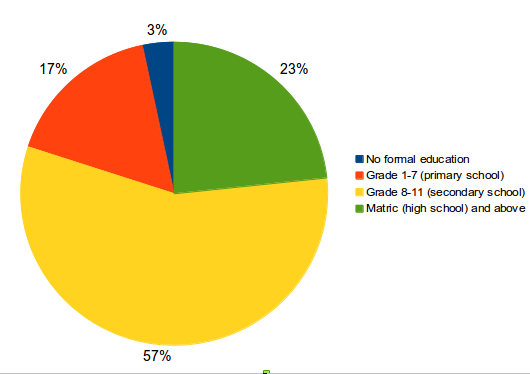
\includegraphics[width=0.6\textwidth]{Figures/education_level.png}
    \rule{35em}{0.5pt}
  \caption{Participants' income distribution.}
  \label{figure:education_level}
\end{figure}

\begin{table}[h!]
  \begin{center}
    \caption{Ethnicity of contextual inquiry's participants}
    \label{table:ethnicity}
	\begin{tabular}{|p{3cm}|p{4cm}|p{2cm}|}
		\hline
		\textbf{Ethnicity}&\textbf{No. of Participants}&\textbf{Percentage}\\
		\hline
		 Black African&8 &26.67\% \\
		\hline
		 Coloured&22& 73.33\%\\
	\hline
	\end{tabular}
  \end{center}
\end{table}

\begin{figure}[htbp]
  \centering
    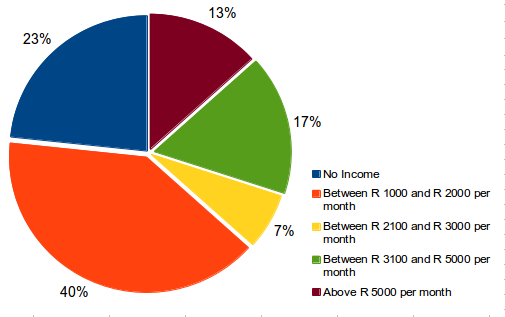
\includegraphics[width=0.6\textwidth]{Figures/income_distr.png}
    \rule{35em}{0.5pt}
  \caption{Participants' income distribution.}
  \label{figure:income_distr}
\end{figure}

Most of them participants were either overweight or obese with an average body mass index (BMI) of 33.36 kg/m\SP{2} (standard deviation of 5.74 kg/m\SP{2}). The average age was 53.13 years old (standard deviation of 11.77 years old).  Almost 86\% (26) were above 40 years of age. This means we were dealing with old participants and hence this group had a tendency of being inexperience with technology.

\section{Data Collection Methods and Analysis}
We used a semi structured questionnaire to interview participants. Each participant was interviewed for a period of 20 to 30 minutes. The questionnaire had four groups of questions and these included demographics: cellphone ownership and utilization; access to information and pedometers; and barriers to diet and physical activity. 

I used both descriptive statistics and qualitative approaches to analyse the information obtained from participants’ responses. Although our objective was to interview overweight and obese patients only but we included few participants who appeared to be thin but were diabetic. Since diabetes is a lifestyle related disease, we found that it would be interesting to also understand utilization of cellphones, and access to information even to individuals who appear not to be overweight but these individuals may had some input on various issues related technology utilization, and  barriers to behaviours that are considered healthy. All the names that are used in presentation of findings are just pseudonyms to protect privacy of participants. 
\section{Findings}
\subsection{Utilization of Cellphones}
Twenty nine out of thirty participants owned cellphones. The most used services were SMS and voice with at least 80\% of the participants using each of the two services. It was found that at least 60\% of the phones owned by participants were smart-phones (Figure \ref{figure:cell_ownership}), but utilization of functionality/services that are supported in smart-phones appeared to be lower relative to voice and SMS (Figure \ref{figure:cell_utilization}). Utilization of smart-phone supported services appeared to decrease with age. Utilization of Whatsapp appeared to be higher compared to other services that are specific to smart-phones. What led to adoption of Whatsapp is that participants were influenced by family members and friends who were already in Whatsapp. These influencers suggested Whatsapp as to be cheaper than SMS. For instance one male participant aged 47 years of age heard that Whatsapp was cheap for communication, and his son helped him on loading it into his phone. Therefore, in this context, social influence played a role in adoption of some smart-phone supported services. There is a positive correlation between social influence and adoption of high-tech innovations \citep{vannoy2010social}.  

\begin{figure}[htbp]
  \centering
    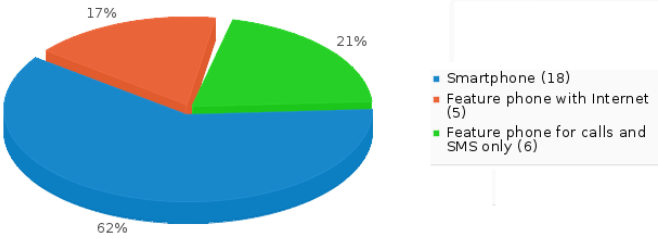
\includegraphics[width=0.5\textwidth]{Figures/cell_ownership.png}
    \rule{35em}{0.5pt}
  \caption{Participants' phones types.}
  \label{figure:cell_ownership}
\end{figure}

\begin{figure}[htbp]
  \centering
    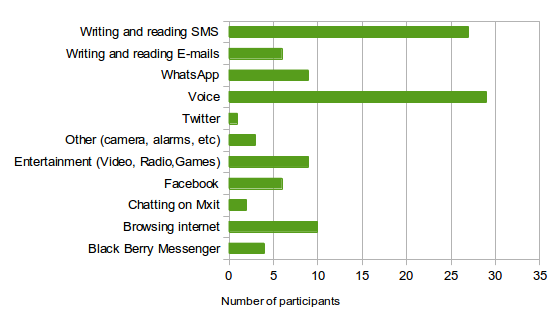
\includegraphics[width=0.5\textwidth]{Figures/cell_utilization.png}
    \rule{35em}{0.5pt}
  \caption{Participants' phones types.}
  \label{figure:cell_utilization}
\end{figure}
\subsection{Help Seeking in Utilization of Cellphones}
There were several scenarios of informal help seeking in utilization of cellphones as highlighted on Table \ref{table:intermediated}. Majority of the participants had solicited  informal help from other people before, in tasks such as: (1) to configure services/apps on their phones (e.g. Whatsapp, Facebook); (2) habituation of skills required for utilization of various functionality (e.g. a phone book of a new or unfamiliar cellphone, Whatsapp); and (3) to interact with certain features such as SMS, Internet browsers, and etc.

There was a variation in the degree of help-seeking and it was determined by how often participants wanted to execute unfamiliar tasks. Tasks such as configuration of services and apps or teaching of individuals had rare occurrences as they only happened when participants had encountered a new application or device and they don't know how to make it functional. 

\begin{table}[h!]
  \begin{center}
    \caption{Scenarios of intermediated interactions}
    \label{table:intermediated}
	\begin{tabular}{|p{1cm}|p{12cm}|}
		\hline
		 \textbf{No.}&\textbf{Scenario}\\
		\hline
		 1& She is being helped to read SMSs by her \emph{daughter}, but she could do it on her own when the daughter is not around. \\
		\hline
		2&He doesn’t know how to reply back to an SMS. So his \emph{grandson} always helps him with that.\\
	\hline
	  3&Her \emph{children} or  \emph{work colleagues} could help her to read SMS written in English that are received through her feature phone. She also mentioned that her two children were skilled in operating cellphone more than her and one of them had a Black Berry smart-phone.\\
	  \hline
	  4&He can take photos using his mobile phone’s camera but he doesn't know how to save those photos on a memory card. His \emph{son} helps him with that once in a while. But, also his son helped him in loading Whatsapp on the phone.\\
	  \hline
	  5&Her \emph{children} have taught her on how to use Whatsapp, take video etc. Now she is learning on how to record sound, set reminders on the phone for insulin and medication.\\
	 \hline
	 6&The \emph{son} would help her to interact with USSD service for checking loyalty points on MTN. MTN is a mobile communication service provider operating in many African countries.\\
	 \hline
	7&She was taught her \emph{son} on how to access a phone-book when composing SMS using her new phone.\\
	\hline
	8&She receives assistance from her \emph{helper} when she wants to send messages to her children.\\
	\hline
	9&She was once helped to do set-up her new phone at a cellphone shop. She was also taught on how to operate BBM by her \emph{grandson}.\\
	\hline
	10& He was once taught on how operate Whatsapp by his \emph{niece}.\\
	\hline
	11&Her \emph{son} and \emph{grandson} have once helped to configure Whatsapp and Facebook on her phone. They have also taught her on how to use those two web services. In addition, she also asks the son to search for certain health information on the Internet, and once the search is done the the son would pass the phone to her to view that information. This happens once in a month.\\
	\hline
	12& Her \emph{son} and \emph{grandson} always teach her on how to use various functionalities like games etc., but she is not so much keen on operating those functionalities. She also admitted that her son and grandson are so much interested with their mobile phones and they spend a lot of time playing using phones something that she doesn't understand.\\
	\hline
	13& This participant didn't own a cellphone. She had no formal education and she was unfamiliar with how to operate a cellphone. Her son receives SMS directed to her and reads it aloud for her or translates an SMS to verbal communication. Also, the son receives phone calls and hands over the phone to her when the person on the other side of the line wants to speak to her.\\
	\hline
	\end{tabular}
  \end{center}
\end{table}
\subsection{Selection of Help Givers}
Participants chose trusted individuals to act as their help givers, typically their children and grandchildren or, less often, children of relatives, family friends, or someone at a cellphone shop. Preference on who is likely to be solicited to assist favours family members. Help givers are selected based on the merit of skills/competence, and interpersonal trust based on a social relationship, and past experience of help seekers on specific help givers.
\subsubsection*{Interpersonal trust}
Interpersonal trust in this context means that whether help-seekers may feel comfortable to seek help from specific people or not. Privacy and existing relationship between a help-seeker and help-giver were first concerns when deciding of who should be asked for help. In additional to that, there was also trust on whether a helper giver may be willing to deliver when solicited for help and this was influenced by experiences in past attempts to seek help. Experiences on past attempt to solicit help refers to help-seekers' positive and negative experiences as an outcome of seeking help. These experiences shaped perceptions of some of the participants towards seeking help with cellphone or any other technology. For instance, one female participant aged 67 years old reported that her daughter helped her once but she had no patience. A male participant aged 47 years of age mentioned that he would like to be assisted on using several services such as MMS, but he thinks that young people may not be having patience to help. Such negative experiences can hinder future help-seeking behaviours from specific help givers. This resonates with the following finding by~\cite{kiesler:twi}, parents may be hesitant to seek informal help from their children after encountering negative experiences.
\subsubsection*{Help-givers' Competence}
In additional to interpersonal trust, the decision of who should be solicited for help was also influenced by help-seekers' level of trust on skills possessed by help-givers. Participants had confidence on competence of their children in using cellphones. Several participants sees their children as having technical know how skills in using cellphones. For instance one 31 years old female participant mentioned that her five years old son knows how to navigate through her whole phone and use it more than what she can do. Another female participant aged 56 years of age explained how children are eager to teach various things on a cellphone but she is not so keen in engaging to cellphones like they way her son and grandson do. A forty seven year of age male participant also mentioned that young people in their families are more skilled in cellphone than old people.
Participants reported that their kids were borrowing their phones to do other tasks and this demonstrated that their kids had better skills with technology. Scenarios of sharing are presented on Table \ref{table:phone_sharing_contextual} below. 

\begin{table}[h!]
\begin{center}
    \caption{Scenarios of sharing of cellphones between participants and their children}
    \label{table:phone_sharing_contextual}
	\begin{tabular}{|p{1cm}|p{12cm}|}
		\hline
		 \textbf{No.}&\textbf{Scenario}\\
	\hline
	1&``Zandile'', a 47 years old female participant, mentioned that her 16 years old son could borrow her phone to use MXit. But herself she is not using anything else on the phone apart from calls and SMS. She also mentioned that she is not so much interested with technology. For example she has internet at work, but she is not really using it.\\
	\hline
  2& ``Buyisiwe'', a 31 years old female participant narrated an experience about her five years old son who uses her smart-phone to listen to music. But she has to lock it while he is listening, because it happened at one point that the son deleted almost everything on the phone.\\
  \hline 
  3&``Celine', a 48 years old female participant lends her phone to her daughter who uses it for normal Internet browsing and Facebook. Celine owned an advanced feature phone enabled with Internet but she was not using internet on the phone.\\
  \hline
	\end{tabular}
  \end{center}
\end{table}
In other scenarios participants mentioned that their kids borrow their phones to search for information related to school assignments. These examples demonstrate the level of skills that potential help-givers can have. Trust on skills possessed by help-givers has been found to be very important to individuals seeking help in the ICTD and HCI contexts.~\cite{ramirez2013infomediaries} suggested that empathy and technical skills of infomediaries influence the outcomes of the process of infomediation to users at public access venues. Another study that examined motivations for informal support in utilization of computers at home found out that skills of help-givers to be one of the factors that influence help-seekers to solicit help from specific people~\citep{poole:chh}. 
\subsection{Access to Health Information and Self-Monitoring Support}
We have collected information about access to health information and self-monitoring support among our participants.The information support in which most the participants relied on is that one provided through face to face meetings with doctors or dieticians during hospital visits. Normal hospital visits are scheduled in intervals of every 3 or six months. But they do visit the hospital only two or three times in a year. In addition to face to face information, patients normally receive paper sheets with information that provide guidance on how to eat healthy. These paper sheets are normally received when patients attend clinic for the first time after being diagnosed with diabetes. Most patients we interviewed were type 2 diabetic and overweight. Doctors and nurses encourage them to eat healthy and exercise. 

Majority of the participant lacked informational support beyond hospital settings that can provide guidance in eating healthy and exercising. Very few participants had used cellphone services as means of querying or receiving information related to health. Only six participant had used internet to search for health information, while only one participant had used a cellphone app for health. Also only two participants had used SMS while only one had used voice to look for health information. Table shows some of the scenarios of where participants had used ICTs in relation to learning about issues concerning their health.
\begin{table}[h!]
\begin{center}
    \caption{Participants’ usage of ICT to fullfil health information needs}
    \label{table:health_information}
	\begin{tabular}{|p{1cm}|p{12cm}|}
		\hline
		 \textbf{No.}&\textbf{Scenario}\\
		 \hline
		 1&``Anitha'', a female participant aged 56 years old, would send SMSs to her son while he is at his workplace. This SMS is usually a request to check for certain  health information on the internet and the son could print for all the material related to that information that was requested. She also follows Dr Oz program on TV about health stuff. If she misses she would go to the Internet and visit the programme's website\\
	  \hline
	  3& ``Jane'', a female participant aged 36 years old, had an app on her phone for giving health tips. She downloaded that app from the Internet.\\
	  \hline
	  4& ``Maria'', a female participant aged 57 years old mentioned that she uses Facebook. She has three diabetic friends and they share diet concerns, recipes, and discuss diabetic specific issues that they experience . They don't discuss about exercise. She sometimes searches on Google about medications especially when she starts using new medications. She uses Google to get more information on the things her doctor advises on.\\
	  \hline
	  5& ``Evelyn'', a female participant aged 63 years old, subscribes to health websites to receive emails with health tips and information. She sometimes calls a dietician to ask about certain diet information.\\
	  \hline
	\end{tabular}
  \end{center}
\end{table}

Self-monitoring of blood glucose seemed to be common among the participants because many of them were diabetic. Self-monitoring of other health parameters such as diet and physical activity seemed not to be done by many participants. Out of thirty participants we interviewed, only two participants had used a pedometer before.  One participant reportedly to use a gym bicycle with a meter that can show distance cycled but she has abandoned using it. Only eight participants reported that they have used a diary before to record the food they have eaten. But this recording is not consistent. Some have stopped doing it although they claim that when they visit hospital, sisters (nurses) always remind them to record foods they have eaten. This food recording is mainly for controlling the levels of blood glucose. For instance, one participant mentioned that she has a note of where she records the blood glucose before she eats and the blood glucose after she has eaten. So she records what she has eaten and the blood glucose levels before and after meals. But overweight and obese diabetic patients are also encouraged to lose weight. Because losing weight has an advantage of lowering levels of blood glucose.  And the only way to lose weight is to follow the recommended diet and become more physically active. 
\subsection{Barriers to Adoption of Healthy Behaviours}
The research teams also examined on barriers to adoption of healthy behaviours such as healthy diet and exercises.

On barriers towards adoption of healthy diet, 76\% of the participants mentioned that the recommended healthy food is always expensive. For instance fat free foods are much more expensive compared to full fat foods. One participant associated eating of certain food cultural upbringing. She explained that Muslims in Cape Town often have very high fat and high sugar content foods  such samosas. One of the comments that appeared to be common to many participants is that; it is difficult to have a budget for separate meals within the family, because diabetic members always have their diet food which seems not be preferred by the rest of the family. So diabetic members might end up eating what the rest of the family eats. They do try to have diet foods by it is not always manageable. But one participant who seemed to be highly motivated disagreed with that argument and said most people lack an understanding of what carbohydrate means. She further mentioned that, education about diet should be contextualized to terms that people are already familiar with. She said most people don't understand what is said by dieticians because it is not communicated in the context they understand. For example the concept of carbohydrates is not well comprehended by many people. But if the topic is well explained using what is already familiar to patients, then they are more likely to comprehend it.

On the question of perceived barriers to physical activity, nine(9) participants mentioned that lack of time to do physical activity because of a busy schedule contributes to less exercising. This is supported by some remarks shared by participants on Table \ref{table:busy_schedules}. Seven participants mentioned that lack of areas to walk around is one of the perceived barriers to physical activity. The most common comment given out to support this argument was that, most of the areas where they live are not safe for somebody to be out walking all the time (Table \ref{table:safety_issues}). Most of these areas have high rates of crime.

\begin{table}[h!]
\begin{center}
    \caption{Excerpts on observation of common participants’ remarks on association between being less active and busy schedules}
    \label{table:busy_schedules}
	\begin{tabular}{|p{2.5cm}|p{10.5cm}|}
		\hline
		 \textbf{Participants}&\textbf{Remarks}\\
	  \hline
	  1&She goes to work very early in the morning and comeback late at night.\\
	  \hline
	  2&Difficult to manage work and household.\\
	  \hline
	  3&She goes to work at 4.00 AM and come back at 7.00 PM. She works for 6 days in a week.\\
	  \hline
	  4&She looks after the family. She takes her sisters child to school, also she does the cooking. She does a lot of house work. So it is difficult to have a planned series of physical activity.\\
	  \hline
	 5&Difficult to balance between planned session for physical activity and manage both work and household at the same time.\\
	 \hline
	 6&Busy with house work at home.\\
	 \hline
	\end{tabular}
  \end{center}
\end{table}

\begin{table}[h!]
\begin{center}
    \caption{Excerpts on observation of participants’ remarks on safety concerns on areas to do walking or running}
    \label{table:safety_issues}
	\begin{tabular}{|p{2.5cm}|p{10.5cm}|}
		\hline
		 \textbf{Participants}&\textbf{Remarks}\\
	  \hline
	  1&The neighbourhood is not safe to wonder around.\\
	  \hline
	  2&It is not safe in her area. She doesn't like to be outside most of the time.\\
	  \hline
	  3&It is unsafe at night and early morning.\\
	  \hline
	  4&The area where she stays is not safe to walk around.\\
	  \hline
	 5&Not safe to walk alone. She prefers to walk through houses.\\
	 \hline
	\end{tabular}
  \end{center}
\end{table}

But despite the claim of lack of both time and areas to exercise these participants mentioned that they been active when doing their daily errands (Table \ref{table:daily_activity}). 

\begin{table}[h!]
\begin{center}
    \caption{Excerpts on observation of participants' remarks regarding physical activities that were part of their daily lives' routines}
    \label{table:daily_activity}
	\begin{tabular}{|p{2.5cm}|p{10.5cm}|}
		\hline
		 \textbf{Participants}&\textbf{Remarks}\\
	  \hline
	  1& She walks from home to visit relatives and friends.\\
	  \hline
	  2&He only walks when he goes to church.\\
	  \hline
	  3&She walks to from her home to a bus station everyday and walks a lot at her work place, so it would be great for her to have something to keep track of how much exercise she gets. She wants to be more active but works 7 days a week.\\
	  \hline
	  4&She exercises in a group of people for three times a week and she now feels much healthier. They have a "biggest loser" competition going at the moment. She would like to have a pedometer to keep a better track of her activity.\\
	  \hline
	 5&She only walks when she has to. She only walks up and down in kitchen. She has a treadmill, but she doesn't use it.\\
	 \hline
	\end{tabular}
  \end{center}
\end{table}

\section{Contextual Design Insights}
These are some of the design insights that were uncovered from the aforementioned findings. In this context, majority of the participants were not utilizing ICTs in self-management of their healthy as they relied only on paper diaries. The only parameter that was being monitored by majority of the participants was blood glucose since all participants were diabetic. Blood glucose is usually controlled through many factors such as diet, exercise, and medication. Type 2 diabetes is linked to obesity and its self-management is mostly through diet and exercise.  The process of self-management can be very cumbersome if it is done using pen and paper and this may reduce compliance \citep{mattila2008mobile}. A paper diary may not be as effective as an electronic diary when it comes into navigating across behaviour patterns for the purpose of self-reflection. Therefore, personal health apps may be important in supporting self-management of health. However, these personal health apps may not be very useful in this context considering the fact that majority of the participants have limited skills in operating technology. The findings above indicate that some participants with limited skills seek help from people with skills. But this approach has its limitations as it relies on existing intrinsic motivation of help givers. Long term usage is crucial for compliance~\citep{mattila2008mobile}, but one cannot achieve this long term usage in the context where a technology needs to be utilized through help givers while most technologies were not designed to anticipate utilization through help givers as part of the usage ecosystem. As it has been advocated that novel approaches such as ICTs in lifestyle modifications may facilitate moving of management of lifestyle-related chronic conditions from healthcare system to citizen-centric health promotion and disease prevention interventions~\citep{korhonen2010personal}; hence it is important for one to think of how we can design technologies that can scale to demographics that are not well-considered in traditional interface design.

Sharing of phones between adults and kids suggests that it is feasible to design a system of which both kids and parents can have access to. What was observed from above is that kids borrow phones because they are motivated with specific things on the phone. One of those things is social media. Therefore if one could design a system that afford specific motivational needs of kids and integrate it with self-monitoring of behaviours of adults then we can enhance motivation kids to help their parents with self-monitoring tasks. With the guidance of self-determination theory, and techniques that have been used in the previous studies that utilized gamification (described on the \emph{Literature Review} chapter), a prototype was developed. The iterations of prototype development and subsequent evaluations are discussed in the next chapters.

\begin{flushright}
\end{flushright}